%!TEX root = mb.tex

% 2nd fig/1st fig = 1.12 ratio
\begin{figure*}[t!]
\centering
\subfigure[Enterprise to external site communication]{
  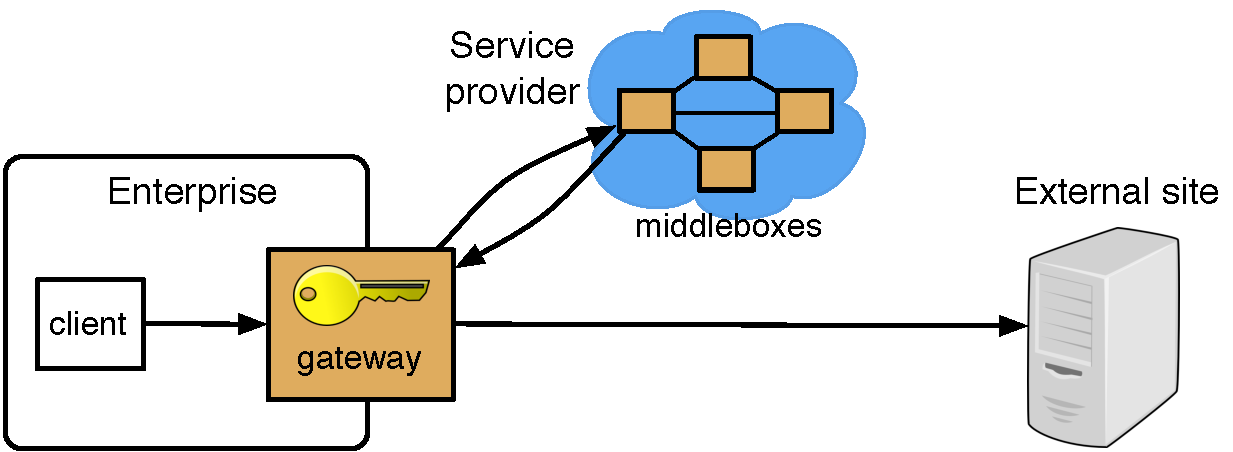
\includegraphics[width=2.8in]{fig/model_1.pdf}
  \label{fig:model1} }
%
\hfill  
\subfigure[Enterprise to enterprise communication]{
   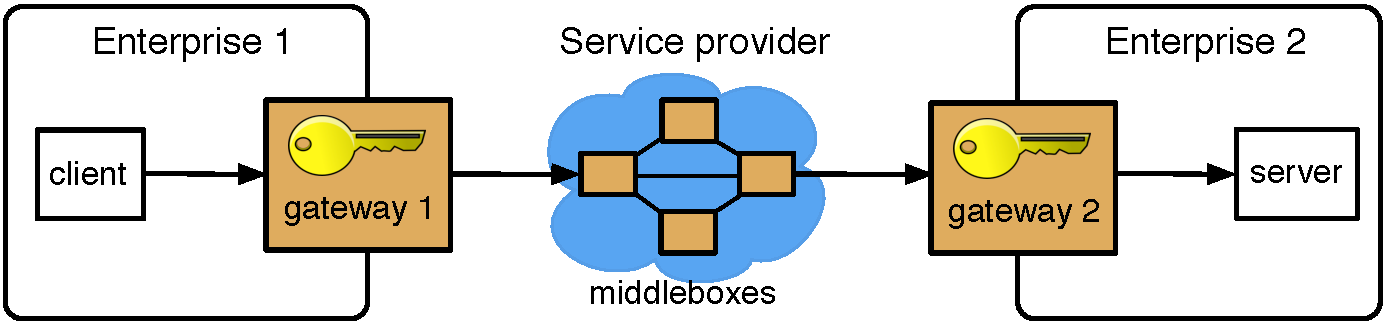
\includegraphics[width=3.2in]{fig/model_2.pdf}
     \label{fig:model2}}
     
     %
\caption{System architecture. Aplomb and NFV system setup with \sys encryption  at the gateway. The arrows indicate traffic from the client to the server; the response traffic follows the reverse direction. \label{fig:sys-overview}}
\end{figure*}




     
\section{Overview}\label{sec:overview}








In this section, we present \sys's architecture, the threat model and applications supported.


% TO CUT REMOVE: just mentino the figures and no need to explain 
\subsection{System Achitecture}

\sys uses the same  architecture as APLOMB, system which redirects an enterprise's traffic to the cloud for middlebox processing~\cite{aplomb}. \sys augments this architecture with confidentiality protection.

The benefits of outsourcing are to delegate the burden of managing and configuring
middleboxes (e.g., upgrading, deciding which vendor to use, monitoring), reduce costs of hardware,
and provide elasticity and fault tolerance; hence \sys should maintain these benefits despite any changes made to to the gateway at the enterprise or middleboxes.
We do not delve further into the details, motivation, and gains of APLOMB's setup, and refer the reader to~\cite{aplomb} for details. 

In the APLOMB setup, there are three parties: enterprise(s), the service provider (SP), and an external site providing
some service. The enterprise runs a gateway (GW) which sends traffic to a middlebox (MB) running in the cloud; in practice this cloud may be either a public cloud service (such as EC2), or an ISP-supported service running at a Central Office (CO).
The service provider -- ISP or cloud-based -- runs a set of middleboxes. 

We illustrate two redirection setups in Fig.~\ref{fig:sys-overview}.  The first setup, in Fig.~\ref{fig:model1},  occurs when the enterprise communicates with an external site: traffic goes to the cloud and back before it is sent out to the Internet. 
It is worth mentioning that APLOMB allows an optimization that saves on bandwidth and latency relative to Fig.~\ref{fig:model1}: the traffic from SP can go directly to the external site and does not have to go back through the gateway. \sys does not allow this optimization fundamentally: the traffic from SP is encrypted and cannot be understood by an external site. We evaluate in \S\ref{sec:eval} what \sys loses by not allowing this optimization. 
Nevertheless, for traffic within the same enterprise, where the key is known by two gateways owned by the same company, we can support this optimization as shown in Fig.~\ref{fig:model2}.




\subsection{Threat Model}

Before defining our threat model precisely, we first provide context and background on the concerns clients have about cloud providers today.

{\bf Context.} 
  Clients adopt cloud services for compute, storage, and increasingly network processing because they the providers are known and trusted to provide good service (at competitive costs). 
  However, while clients trust cloud providers to perform their services correctly, there is increasing concern that cloud providers may access or leak confidential data in the process of providing service.
  Reports in the popular press describe companies selling customer data to marketers~\cite{example}, disgruntled employees snooping or exporting data~\cite{something}, and hackers gaining access to clouds~\cite{somethingelse}.
  The type of threat in this scenario is referred to as an `honest but curious' or `passive'~\cite{goodrich} attacker: a party who is trusted to handle the data and deliver or service it correctly, but who may want to learn more from the data than is strictly necessary or desired.
  Such an attacker differs from a classical, `active' attacker, who seeks to harm the client outright, for example by manipulating data or denying service~\cite{goodrich}.
  This distinction, which based on users concerns today, informs our threat model below. 

{\bf Threat Model.}
The goal of \sys is to protect the privacy of the traffic against an attacker at the service provider  
(cloud employee, or hacker gaining access to cloud machines). 
We consider a strong  attacker, one that has gained access to {\em all the data at SP}.
This includes any traffic and communication SP receives from the 
gateway, any logged information, cloud state, and so on. Nevertheless, we assume that 
SP provides good service and runs middlebox functionality correctly -- but we do not want SP to 
see the traffic in the process of doing so.  

We assume that the gateways are managed by the enterprise and hence trusted; in particular,  they do not leak information.


Some middlebox functionalities (such as intrusion or exfiltration detection) have a threat model
of their own about the client and the server. For example, intrusion detection assumes that 
the client or the server could misbehave, but at most one of them misbehaves~\cite{Bro}.  
%(indeed, if both misbehave, they can send attack traffic to each other encrypted with a shared symmetric key and fundamentally
%no one can detect such an attack).  
We preserve these threat models unchanged. These applications rely
on the middlebox to detect attacks in these threat models. Since we assume the middlebox executes
its functions correctly and \sys preserves the functionality of these middleboxes, 
these threat models are irrelevant to the protocols in \sys, and we will not discuss them again. 

\textbf{In comparison to BlindBox and APLOMB.}
APLOMB~\cite{aplomb} assumes that the provider is fully trusted with client data; \sys's threat model allows for a passive attacker with access to the clients' data at the cloud.
The differences between BlindBox~\cite{blindbox} and \sys are threefold:

%
\noindent(1) With BlindBox, the middlebox and client are unknown to each other; the middlebox wishes to {\it enforce} a policy over the client's traffic, and the client is not allowed to observe the rules being enforced. With \sys, the policy imposed over a clients traffic is a policy the client {\it wishes to have enforced}. 
Some rules may come from the client itself -- such as exfiltration policies -- while others may come from a trusted rule provider such as McAfee or Symantec, as in BlindBox. We discuss how rules are generated and exchanged between the gateway and the cloud in \S\ref{sec:gateway}.
An additional consequence of this shift -- that the client now desires that the policy be enforced properly -- is that BlindBox requires some validation that the client has not attempted to evade proper encryption, whereas our client is trusted to faithfully operate the protocol.
%

\noindent(2) Under \sys, the gateway is trusted by all end hosts at the enterprise network; it performs encryption on their behalf. This gives \sys deployability benefits relative to BlindBox -- only one gateway needs to be upgraded to support the new protocol, not every end host on the network. It also gives performance benefits: where BlindBox incurs a costly setup operation of around 97s for every connection, this setup occurs {\it once} at the gateway under \sys to establish a persistent connection shared by all end hosts. This is only possible because the gateway exists as a trusted intermediary in the network.

\noindent(3) BlindBox provides privacy guarantees comparable to SSL: a middlebox will observe packet headers, but not payload contents. \sys provides stronger privacy coverage, comparable to IPSec in that it obscures all packet headers as well as payloads.

%
%
\subsection{Encryption Overview}
\eat{
\begin{figure}[t!]
\centering
  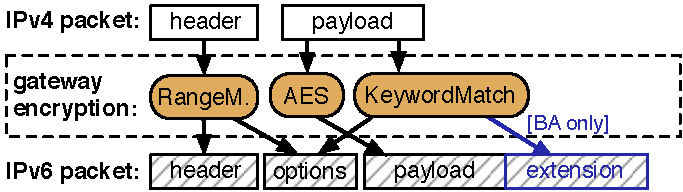
\includegraphics[width=3.0in]{fig/packet.pdf}
\caption{Packet encryption at the gateway. Patterned squares indicate encrypted data. Only for DPI  middleboxes,  KeywordMatch produces additional encrypted data. \justine{Change fig to say DPI not BA}  \label{fig:packet}}
\end{figure}
}

\begin{figure*}[t!]
\centering
  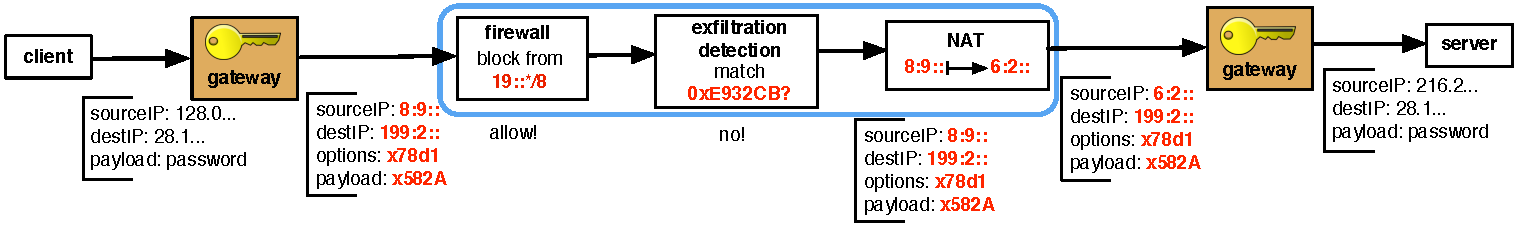
\includegraphics[width=6.7in]{fig/packetpath.pdf}
\caption{Example of packet flow through a few middleboxes. Red in bold indicates encrypted data. \label{fig:packetflow}}
\end{figure*}



To protect privacy , \sys encrypts all traffic passing through the service provider (SP).
\sys encrypts IP addresses, ports, and the payload of the packet.
As in Fig.~\ref{fig:sys-overview}, the gateway has a secret key $k$; in the setup with two gateways, they share
the same secret key. The gateway encrypts all traffic going to the service provider using \sys's encryption schemes.
The middleboxes at SP process {\em encrypted traffic} using \sys's protocols. 
To perform detection, the service provider uses a set of {\it encrypted rules} that allow it to perform comparisons against the encrypted values it observes in the traffic.
After the processing, the middleboxes
will produce encrypted traffic which SP sends back to the gateway. The gateway decrypts the traffic using the key $k$.

Throughout this process, middleboxes at SP handle only encrypted traffic and never access the decryption key. This ensures
that an attacker that steals all the data from SP will  see only encrypted traffic, which protects the privacy of the 
traffic. 
On top of \sys's encryption, the gateway can use a secure tunneling protocol, such as SSL or IPSec to secure the communication to SP.

\begin{table}
\centering
\small
\hspace{-2pt}
\begin{tabular}{l|l|p{.45in}|p{.45in}|p{.45in}}
&{\bf MB}&{\bf TCP/IP Header}&{\bf HTTP Headers}&{\bf Byte Stream}\\

\hline

\parbox[t]{1mm}{\multirow{3}{*}{\rotatebox[origin=c]{90}{Header}}}
&IP Firewall&Range&-&-\\
&L4 LB&Range&-&-\\
&NAT&Exact&-&-\\
\hline


\parbox[t]{1mm}{\multirow{2}{*}{\rotatebox[origin=c]{90}{DPI}}}
&IPS&Range&Exact&Exact\\
&Exfiltration&Range&Exact&Exact\\
\hline

\parbox[t]{1mm}{\multirow{3}{*}{\rotatebox[origin=c]{90}{HTTP}}}
&Proxy&Exact&Exact&-\\
&Parent Filter&-&Exact&-\\
&L7 LB&Exact&Exact&-\\
\hline
*&VPN&-&-&-\\

\end{tabular}
\caption[]{Middleboxes supported by \sys and categorized as Header, DPI, or HTTP middleboxes depending on what fields they access. Middleboxes are also labeled whether they perform `exact match' comparisons against rules, or `range match' comparisons against rules.\label{tbl:mbreqs}}

\end{table}



\noindent\textbf{Packet encryption}
Recall that the provider holds a set of encrypted rules at the middleboxes which it uses to operate over the client's encrypted traffic.
\sys uses three encryption schemes to protect data privacy while allowing comparison against encrypted rules at the cloud: 
\begin{myitemize}
\item Traditional AES: provides strong security and no computational capabilities)
\item KeywordMatch:  allows the provider to detect if an encrypted value in the packet is equal to an encrypted rule value
\item RangeMatch: allows the provider to detect whether or not an encrypted value lies in a range of rule values -- e.g. addresses in 128.0.0.0/24 or ports between 80-96.
\end{myitemize}
We discuss these cryptographic algorithm in \S\ref{sec:buildingblocks}.

The key idea behind \sys is to encrypt {\it each field} of a packet using the appropriate encryption algorithm such that middleboxes can process each field of data as if it were not encrypted. 
Plaintext packets are encrypted, field-by-field, to generate a new IPv6 packet that is processed at the cloud.
For example, an encrypted IPv6 packet will contain a source address that is an encryption of the original packet's source address using RangeMatch. This allows, e.g., a firewall to check whether the packet's source belongs to a prefix known to be controlled by a botnet -- but without learning what the actual source IP address is.
We use IPv6 at the cloud because our RangeMatch scheme requires 128 bits to encode an encrypted IP address -- and because we expect more and more service providers to be moving to IPv6 by default in the future.
This is a trivial requirement to impose, as it is easy to convert from IPv4 to IPv6 (and back) at the gateway~\cite{6to4,4to6}; clients may continue using IPv4 and the tunnel connecting the client to the provider may be either v4 or v6.

We choose which encryption scheme is appropriate for each field based on a high level classification of middlebox capabilities.
Table~\ref{tbl:mbreqs} shows a list of all middleboxes supported by typical outsourcing deployments~\cite{aplomb} and their processing requirements.
We classify these middleboxes as operating only over packet headers, operating only over packet headers and HTTP headers, or operating over all data including arbitrary fields in the connection bytestream (DPI).
We revisit these middleboxes in detail in \S\ref{sec:mbs}.


{\bf Example.} Fig.~\ref{fig:packetflow} shows the end-to-end flow of a packet through three example middleboxes in the cloud, each middlebox operating over an encrypted field.  
First,  the gateway encrypts the packet as explained above. The packet passes through the firewall which tries to match the encrypted information from the header against its encrypted rule, and decides to allow the packet. Next, the exfiltration device checks for any suspicious (encrypted) strings on the extension of the packet's payload, and not finding any, it allows the packet  to continue to the NAT. The NAT maps the source IP address to a different IP address. Back at the gateway, the gateway decrypts the packet. 



